\documentclass[a4paper,11pt]{article}

\usepackage[T1]{polski}
\usepackage[utf8]{inputenc}
\usepackage{amsmath}
\usepackage{amssymb}
\usepackage{graphicx}

\hoffset=-3.0cm                 
\textwidth=18cm                
\evensidemargin=0pt
\voffset=-3cm                  
\textheight=27cm                
\setlength{\parindent}{0pt}             
\setlength{\parskip}{\medskipamount}    
\raggedbottom                           

\title{Grafika komputerowa \\
{Zadanie 3}}
\author{Nowak Piotr, Smoliński Mateusz}
\date{maj 2022}

\begin{document}
\maketitle

\section{Realizacja zadania}
Zadanie zostało wykonane w środowisku python z użyciem biblioteki 
pygame. Zrealizowany został model odbicia światła Phonga. 
W centrum widoku umieszczona jest 
nieruchoma kula o zadanym promieniu. Umiejscowienie źródła światła 
i niektóre parametry można zmieniać w trakcie działania programu.
Ponownie obliczone oświetlenie pojawi sie na ekranie po chwili od 
zadania zmiany.

\section{Kula}
Powierzchnia kuli reprezentowana jest jako zbiór punktów 
spełniających równanie \(x^2 + y^2 + z^2 < 1\), gdzie \(z \geqslant 
0\). Początkową barwa każdego piksela obrazu jest pełna czerń. 
Dla każdego z punktów obrazu należącego do kuli, czyli 
spełniającego równanie \(x^2 + y^2 < 1\) obliczane jest  
kolejnych rodzajów światła według opisu w kolejnych 
akapitach.

\section{Światło otoczenia (ambient)}
Jest to stałe jednakowe oświtlenie całej powierzchni. Obliczane jest 
dla każdego piksela za pomocą wzoru: \(I_a = k_a * i_a\), gdzie \(k_a\) 
jest stałą odbicia światła otoczenia, a \(i_m\) jest kolorem światła.
\begin{center}
    
\includegraphics[width=0.3\columnwidth]{ambient.png}
\end{center}

\section{Światło rozproszone (diffuse)}
Jest to oświetlenie wynikające z kąta padania promieni światła 
na powierzchnię. Natężenie jest maksymalne kiedy powierchnia jest 
ustawiona prostopadle to padającego na nią promienia, a minimalne 
(zerowe) kiedy kąt jest większy lub równy kątowi prostemu. Obliczane 
jest to wzorem: \(I_d = k_d * (\hat{L}_m  \cdot \hat{N} ) * i_d\), 
gdzie \(k_d\) jest stałą odbcia światła rozproszonego, \(\hat{L}_m\) jest 
znormalizowanym wektorem skierunkowanym z danego punktu do źródła 
światła, \(\hat{N}\) jest wektorem znormalizowanym wektorem normalnym 
z tego puntu powierzchni, a \(i_d\) jest kolorem światła. \\
Punkt \(p = (x, y, z)\) powierzchni w danym pikselu obrazu otrzymujemy 
ze wzoru \(z = \sqrt{1 - x^2 - y^2} \), dla zadanych x, y. Wektor 
normalny jest równy wektorowi od środka układu do tego punktu.
\begin{center}
    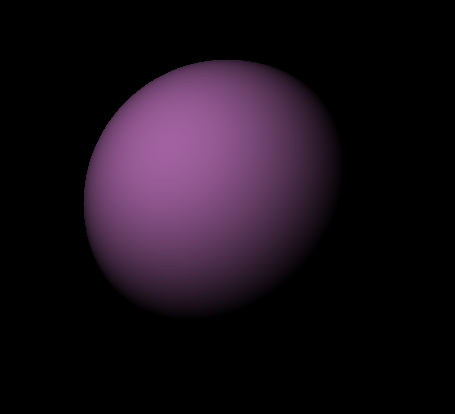
\includegraphics[width=0.3\columnwidth]{diffuse.png}
\end{center}

\section{Światło odbite kierunkowo (specular)}
Jest widoczne dla powierchni błyszczących. Obliczane jest za pomocą 
wzoru: \(I_s = k_s * (\hat{R}_m  \cdot \hat{V} )^\alpha * i_s\), 
gdzie \(k_s\) jest stałą odbcia światła specular, \(\hat{R}_m\) jest 
znormalizowanym wektorem światła odbitego od powierzchni od danego 
punktu ze źródła światła, \(\hat{V}\) jest wektorem znormalizowanym 
wektorem od punktu do punktu obserwatora (kamery), \(\alpha\) jest
stałą błyszczenia danej powierzchni, a \(i_s\) 
jest kolorem światła (w zadaniu białe).
\begin{center}
    
\includegraphics[width=0.3\columnwidth]{specular.png}
\end{center}

\section{Pełny obraz}
Wartości każdego rodzaju światła dla danego piksela są dodawane do 
siebie, ograniczane przez minimalne i maksymalne wartości RGB i 
wyświetlane na ekranie.


\section{Działanie programu}
Podczas działania programu można wybrać jeden z trzech zestawów 
parametrów wciskając przyciski 1, 2 lub 3 na klawiaturze. Można 
też zmienić umiejscowienie źródła światła klikając kursorem w pozycję 
na ekranie.

\begin{center}
    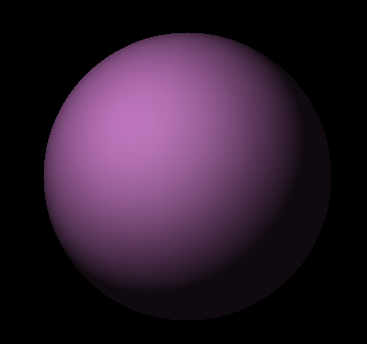
\includegraphics[height=0.27\columnwidth]{full1.png}
    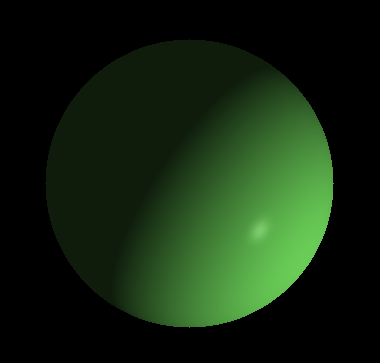
\includegraphics[height=0.27\columnwidth]{alt2.png}
    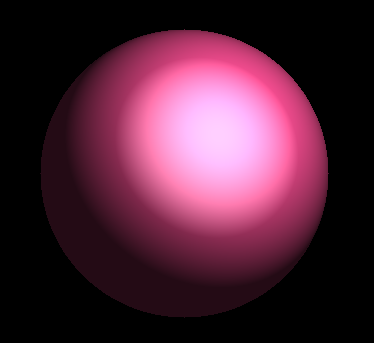
\includegraphics[height=0.27\columnwidth]{alt3.png}
\end{center}
\end{document}